\scanpage{128}
% archive sheet number: 127
% source lines 1--10
$B_{\handwritten{\alpha}}$ sur les $A_{\handwritten{\alpha}}^{\handwritten{'}}$ qui se réduisent les unes en les autres \ldots), \deleted{les $B$} de plus chaque $B_{\handwritten{\alpha}}$ étant coplat sur $A_{\handwritten{\alpha}}$. La structure\inserted{\handwritten{$c$}}\handwritten{\begin{tikzpicture}[x=.35cm,y=.35cm,baseline=-.2ex]\draw (.15,-.5) .. controls (-.2,-.15) and (.4,.1) .. (.2,.4) .. controls (.1,.55) and (.1,.65) .. (.4,.7);\end{tikzpicture}} précédente revient à un isomorphisme de \uline{b\deleted{i}}\deleted{m}\inserted{co}\uline{odules} sur \deleted{$\unsure{B'|A'}\unsure{\otimes|\Omega}_{k}$} $A'$
\[
\begin{array}{l@{\qquad}l}(*)&B\otimes_{k'}B\handwritten{\unsure{\overset{\sim}{\Longleftarrow}|\xleftarrow{\sim}}}B\otimes_{k'}A'.\quad\deleted{\text{\unsure{De|En}}}\end{array}
\]
$\unsure{\rlap{\(\mathrm u\)}U|\mathbb U}$tilisant l'augmentation du facteur $A'$, on en conclut un homomorphisme
\[
\begin{array}{l@{\qquad}l}(**)&B\otimes_{k'}B\handwritten{\longrightarrow}B\end{array}
\]
qui sera un \uline{homomorphisme de comodules} sur $A'$ (NB utiliser la multiplication de $A'$ pour définir la structure de $A'$-comodule sur le produit tensoriel sur $k$ de deux tels), i.e. on a une loi de composition sur $B$ ``compatible avec la structure de $A'$-comodule''.
\margin{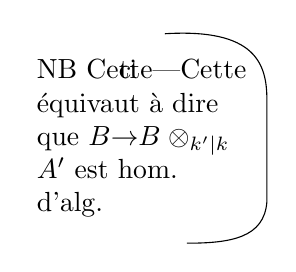
\begin{tikzpicture}[x=.35cm,y=.35cm,baseline=(n.base)]\node[anchor=north west,align=left,text width=2.7cm] (n) at (0,0) {NB \unsure{Ce\rlap{c}t\rlap{i}t\deleted{e}|Cett\deleted{e}} équivaut à dire que $B\handwritten{\to}B\otimes_{\unsure{k'|k}}A'$ est hom. d'alg.};\draw (5.0,.6) .. controls (8.3,.8) and (8.7,-.5) .. (8.7,-1.8)--(8.7,-5.5) .. controls (8.6,-6.8) and (7.4,-7.0) .. (5.8,-7.0);\end{tikzpicture}}
\margin{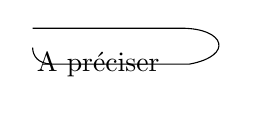
\begin{tikzpicture}[x=.35cm,y=.35cm,baseline=(n.base)]\node[anchor=north west,align=left] (n) at (0,0) {A préciser};\draw (.2,.5)--(5.6,.5) .. controls (7.2,.5) and (7.5,-.5) .. (5.9,-.8)--(.9,-.8) .. controls (.4,-.8) and (.2,-.5) .. (.2,-.2);\end{tikzpicture}}\margin{\handwritten{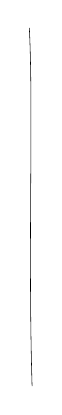
\begin{tikzpicture}[x=.35cm,y=.35cm,baseline=-.2ex]\draw[line width=.2pt] (0,0) .. controls (.15,-3) and (-.05,-8) .. (.1,-13);\end{tikzpicture}}}
\margin{
\begin{tikzpicture}[x=.35cm,y=.35cm,baseline=(n.base)]\node[anchor=north west,align=left,text width=5.6cm] (n) at (.6,0) {Sauf erreur, la donnée de\\(*) \uline{équivaut} \uline{à celle de}\\(**)};\draw[line width=.5pt] (0,.2)--(0,-2.9);\draw[line width=.5pt] (.22,.3)--(.22,-2.8);\end{tikzpicture}}

% source lines 11--27
Si $\handwritten{\Delta}$ sur $U$ est unitaire i.e. $A$ est unitaire i.e. le $\otimes$ sur $X$ \deleted{est adme \illegible{1}} admet une unité bilatère compatible avec $F$, alors la compatibilité de $c$ avec les unités s'exprime, sauf erreur, par la condition que la loi de composition (**) est unitaire.\deleted{(} En effet, il faut écrire que l'on a un isomorphisme \deleted{$L\otimes_{\handwritten{U}}k$} $L\otimes_{U'}k'\handwritten{\simeq}k'$ satisfaisant certaines conditions, or cela revient à se donner un\deleted{e élément de} augmentation de $L$ satisfaisant une certaine condition (savoir \deleted{être compatible avec}\inserted{être unité bilatère pour} la structure diagonale de $L$) ou encore un élément de $B$ qui es t une unité bilatère.\inserted{Ceci implique aussi que $B$ est \uline{fidèlement} plat sur $k'$.}\handwritten{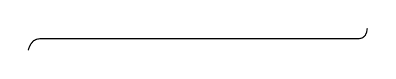
\begin{tikzpicture}[x=.35cm,y=.35cm,baseline=-.2ex]\draw (0,-.3) .. controls (.1,.05) and (.25,.12) .. (.45,.12)--(12.0,.12) .. controls (12.2,.12) and (12.3,.3) .. (12.3,.5);\end{tikzpicture}}\handwritten{\begin{tikzpicture}[x=.35cm,y=.35cm,baseline=-.2ex]\draw[line width=.5pt] (0,.05) .. controls (1,-.15) and (1.4,.3) .. (1.3,.7);\end{tikzpicture}} De même, si $\handwritten{\Delta}$ est associatif, i.e.\inserted{si}\handwritten{
\begin{tikzpicture}[x=.35cm,y=.35cm,baseline=-.2ex]\draw (0,.5) .. controls (-.2,0) and (.1,-.4) .. (.4,-.2)--(1,-.2) .. controls (1.3,-.2) and (1.1,.2) .. (1.4,.35);\end{tikzpicture}} on a pour $\otimes$ une d\deleted{t}onnée d'associatilité $\handwritten{\phi}$ compatible avec $F$, alors $c$ est compatible avec celle-ci sss $B$ est une algèbre associative. \deleted{Quand les deux conditions sont vérifi} Enfin, quand $\handwritten{\Delta}$ est commutative i.e. $C$ avec $\handwritten{\psi}$ donnée de symétrie, \ldots\ alors $c$ est compatible avec cette dernière, et la donnée de symétrie habituelle sur $\unsure{\mathrm{P}\rlap{\(\mathrm r\)}\mathrm o\rlap{\(\mathrm r\)}\mathrm o\mathrm{jf}|\mathrm{Poojf}}(k')$ sss la loi de composition de $B$ est \deleted{asso} commutative. \handwritten{[}(Mais alors, en termes du monoïde affine $\handwritten{\unsure{\rlap{\(G\)}H|H|G|\mathscr{H}|\mathscr{G}}}$ défini par $A$ sur $k$, on voit que les structures de $B$ s'expriment en termes de\inserted{\handwritten{$P:$}}\handwritten{\begin{tikzpicture}[x=.35cm,y=.35cm,baseline=-.2ex]\draw (0,-.3)--(.4,-.15)--(1.3,.9);\end{tikzpicture}} $\mathrm{Spec}\ B$ en disant que $\handwritten{{\rlap{\(G\)}H}_{k'}}$ y opère à droite,\inserted{\handwritten{et $P$ est form.\textsuperscript{\handwritten{\begin{tikzpicture}[x=.35cm,y=.35cm,baseline=-.2ex]\draw[line width=.4pt] (.08,.35)--(.06,.1) .. controls (.05,.02) and (.09,-.02) .. (.13,.01);\end{tikzpicture}}} princ. hom.}}\handwritten{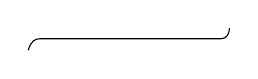
\begin{tikzpicture}[x=.35cm,y=.35cm,baseline=-.2ex]\draw (0,-.3) .. controls (.1,.05) and (.25,.12) .. (.45,.12)--(7.0,.12) .. controls (7.2,.12) and (7.3,.3) .. (7.3,.5);\end{tikzpicture}} et on voit de plus qu'après le changemen\unsure{t}
\margin{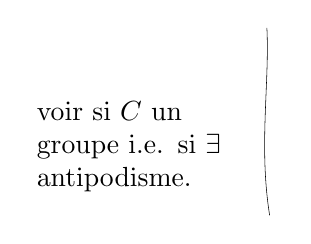
\begin{tikzpicture}[x=.35cm,y=.35cm,baseline=(n.base)]\node[anchor=north west,align=left,text width=3.0cm] (n) at (0,0) {\handwritten{voir si $C$ un groupe i.e. si $\exists$ antipodisme.}};\draw[line width=.2pt] (8.7,2.3) .. controls (8.8,.3) and (8.4,-2.0) .. (8.8,-4.5);\end{tikzpicture}}
